\documentclass[a4paper,10pt]{scrartcl}

\usepackage{amsmath,amsfonts,amssymb} % mathematical environments, symbols and fonts
\usepackage[utf8]{inputenc}           % input encoding of utf8 source files
\usepackage{graphicx}                 % including graphics
\usepackage[english]{babel}           % babel package for hyphenation (choose your language from english, ngerman)
\usepackage{booktabs}                 % more beautiful tables
\usepackage{cite}                     % allow citations
\usepackage{url}                      % including URLs
%\usepackage{subfigure}                % including subfigures
\usepackage{caption}
\usepackage{subcaption}
\usepackage{hyperref}
% Package for including code in the document
\usepackage{listings,relsize} 
\usepackage{color}
\usepackage{colortbl} 		%para colorear tablas

\definecolor{dkgreen}{rgb}{0,0.6,0}
\definecolor{gray}{rgb}{0.5,0.5,0.5}
\definecolor{mauve}{rgb}{0.58,0,0.82}

%lstloadlanguages{R}
%lstloadlanguages{Java}
\lstloadlanguages{C}
\lstset{language=C}

\lstset{
  keywordstyle=\color{blue},
  commentstyle=\color{gray},
  stringstyle=\color{red},
  basicstyle=\ttfamily\small,
  numbers=left,		% where to put the line-numbers; possible values are (none, left, right)
  numbersep=7pt,	% how far the line-numbers are from the code
  numberstyle=\ttfamily\color{gray}\footnotesize, % the style that is used for the line-numbers
  firstnumber=1,
  stepnumber=1,		% the step between two line-numbers. If it's 1, each line will be numbered
  columns=fullflexible,
  frame=single,		% adds a frame around the code
  breaklines=true,
  showstringspaces=false,
  basewidth={0.5em,0.4em}
}

\usepackage{fancyhdr}
%\setlength{\headheight}{15.2pt}
\setlength{\headheight}{22.6pt}
\pagestyle{fancy}


% =======================================================================
% Begin of the document

\begin{document}

\lhead{Jon Udaondo}
\chead{}
\rhead{Gamestore}

% =======================================================================
% Title and author list
\title{Proyecto \\ Gamestore}  % title
%\titlerunning{Kurztitel}            % abbreviated title (for running head)
\author{Jon Udaondo}       % author name
\date{Abril, 2014}
%\institute{University of Vienna\\Faculty of Computer Science\\
%\email{moritz.reincolacoca1hardt@univie.ac.at}
\maketitle
\begin{figure}%[htb!]
\centering

\includegraphics[width=0.5\textwidth] {tituloo.png}
%\caption{}
\label{fig:titulo}
\end{figure}

\renewcommand{\tablename}{Tabla}
\renewcommand{\lstlistingname}{Código}
\renewcommand{\contentsname}{Contenido}
\renewcommand{\figurename}{Fig.}
\renewcommand{\refname}{Referencias}
\pagebreak
\tableofcontents
%\pagebreak

% \begin{abstract}
% This document contains all assumptions I made during this task.
% \end{abstract}

\pagebreak
\section{Subiendo la aplicación a AWS}
\subsection{Creando una máquina virtual en EC2}
\begin{enumerate}
	\item Lo primero que tenemos que hacer es registrarnos en \emph{Amazon Web Services (AWS)} para ello vamos a \url{http://aws.amazon.com/es/free/} y pulsamos en ``Comience de forma gratuita''. 
	\item Introducimos nuestros datos personales y nos pedirá introducir nuestra tarjeta de crédito. En el siguiente paso nos saldrá un número de validación en pantalla el cual tendremos que introducir en nuestro móvil tras recibir una llamada de Amazon. 
	\item Posteriormente llegaremos a una pantalla en la que tendremos que seleccionar el plan de soporte (fig. \ref{fig:plan_soporte}). Seleccionaremos ``Basic (gratuito)''.
	\begin{figure}[htb!]
		\centering
		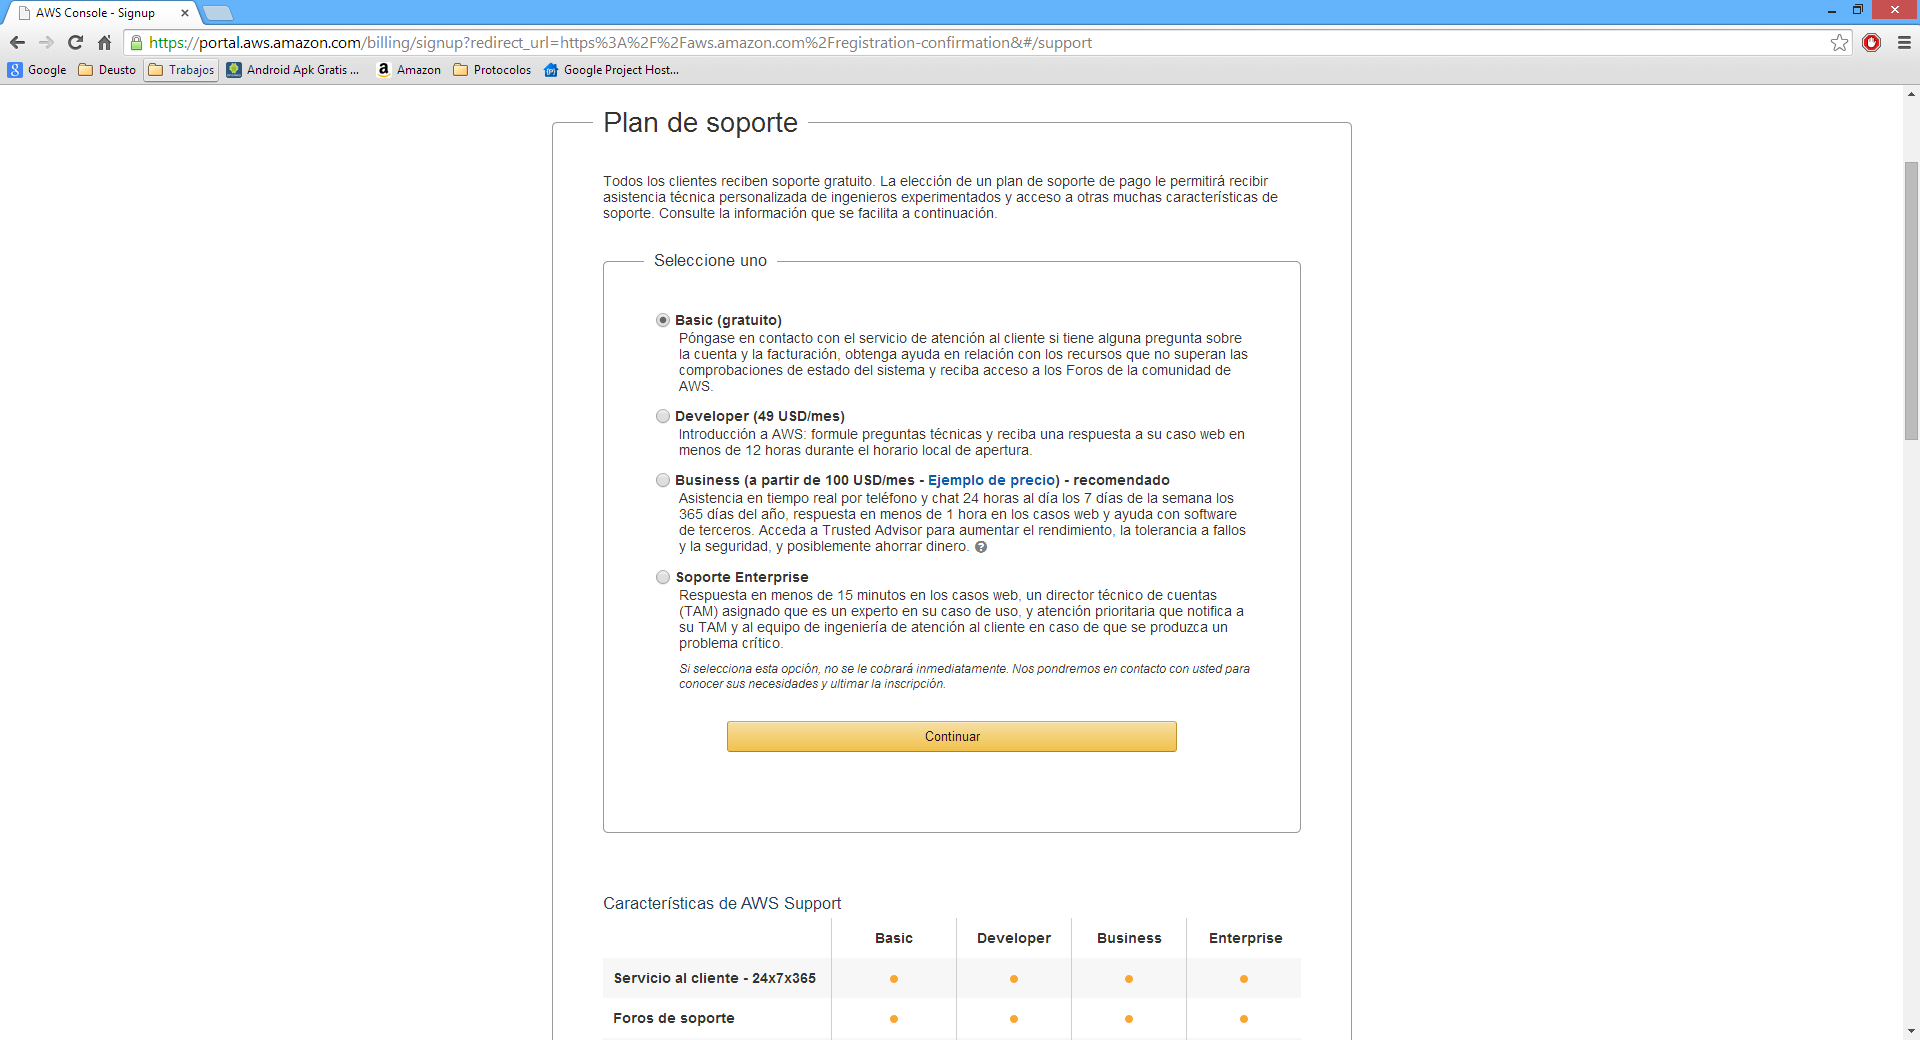
\includegraphics[width=0.8\textwidth] {plan_soporte.png}
		\caption{Plan de soporte}
		\label{fig:plan_soporte}
	\end{figure}
	\item Una vez finalizado ya abremos acabado de registrarnos.
	\item Tendremos que dirigirnos a ``Mi cuenta/Consola'' y seleccionar ``AWS Management Console'' (\url{https://console.aws.amazon.com/console/home?region=us-west-2}). En esta página veremos lo que hay en la figura \ref{fig: amc}.
	\begin{figure}[htb!]
		\centering
		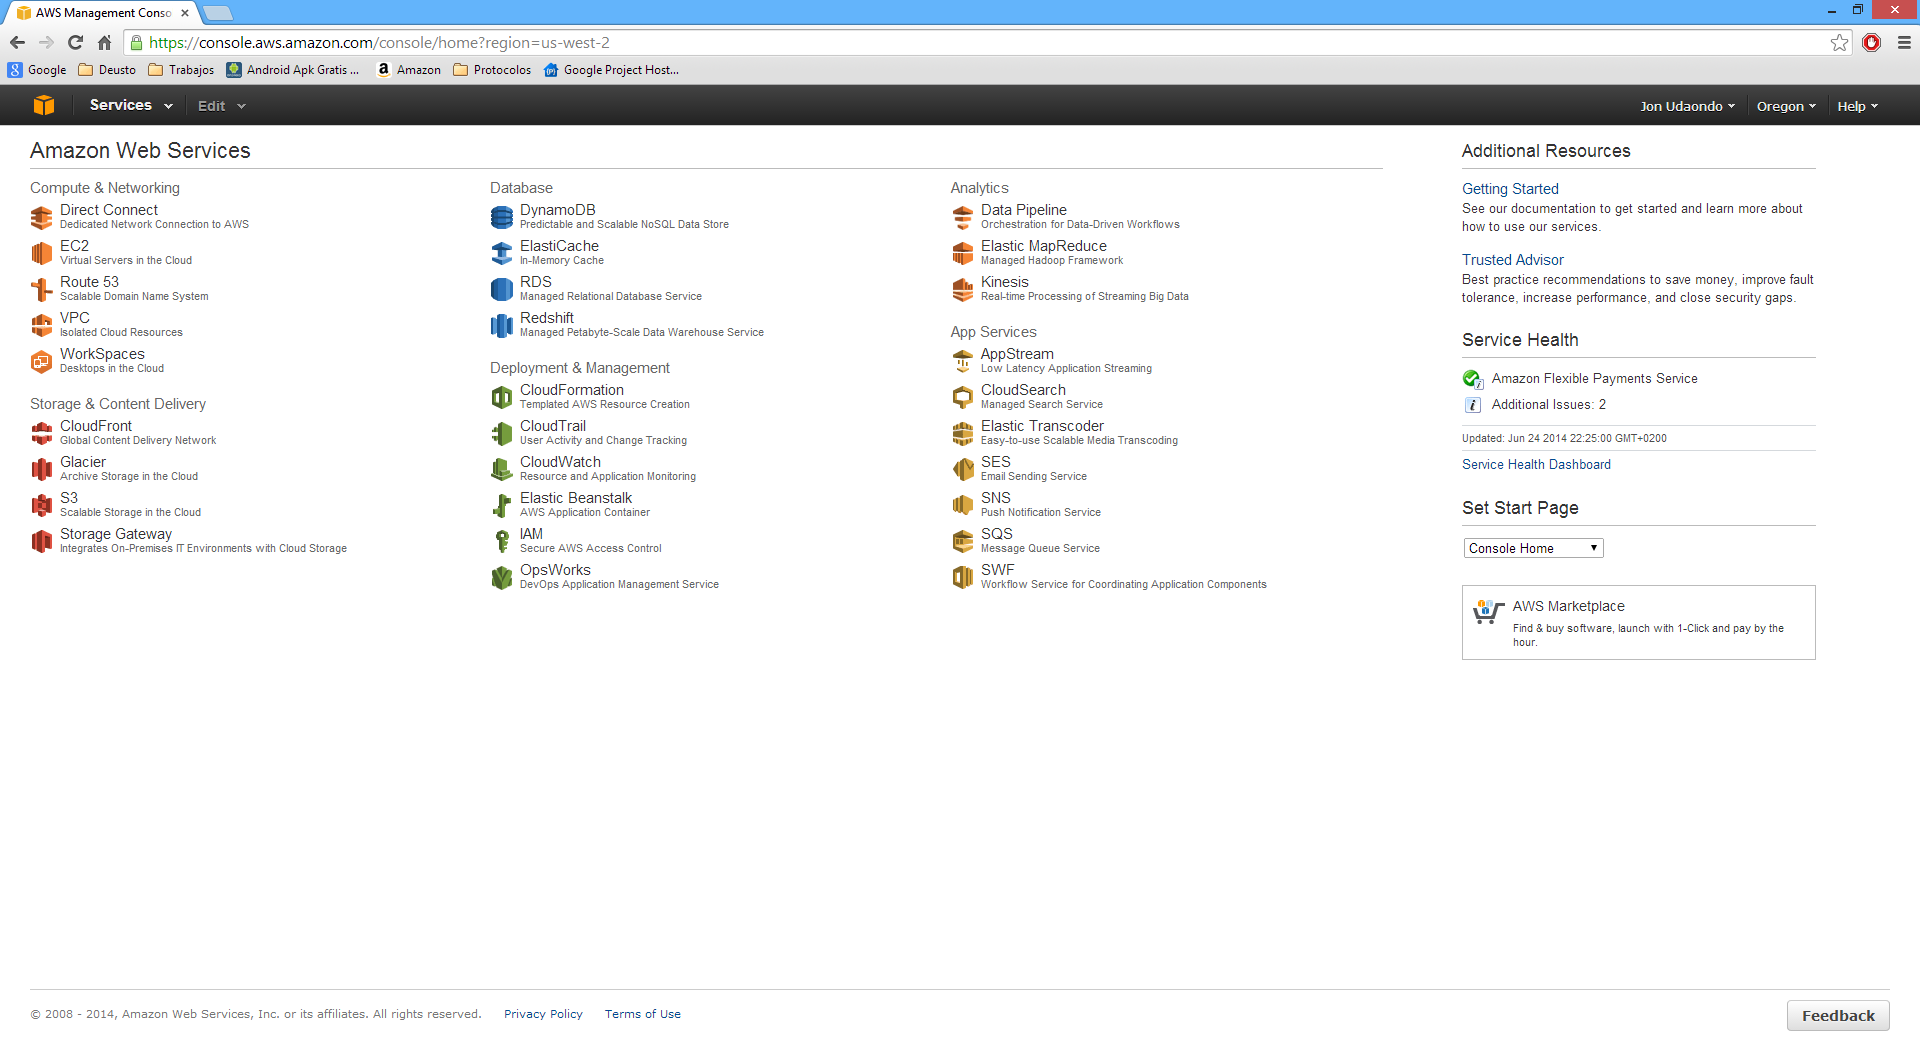
\includegraphics[width=0.8\textwidth] {amc.png}
		\caption{Amazon Management Console}
		\label{fig: amc}
	\end{figure}
	\item Seleccionamos ``EC2 (Virtual Servers in the Cloud''). 
	\item Nos saldrá una lista con bastantes máquinas virtuales que Amazon las llama ``Amazon Machine Image (AMI)'' (fig. \ref{fig: ami}). Elegiremos la máquina virtual de Ubuntu (64bits).
	\begin{figure}[htb!]
		\centering
		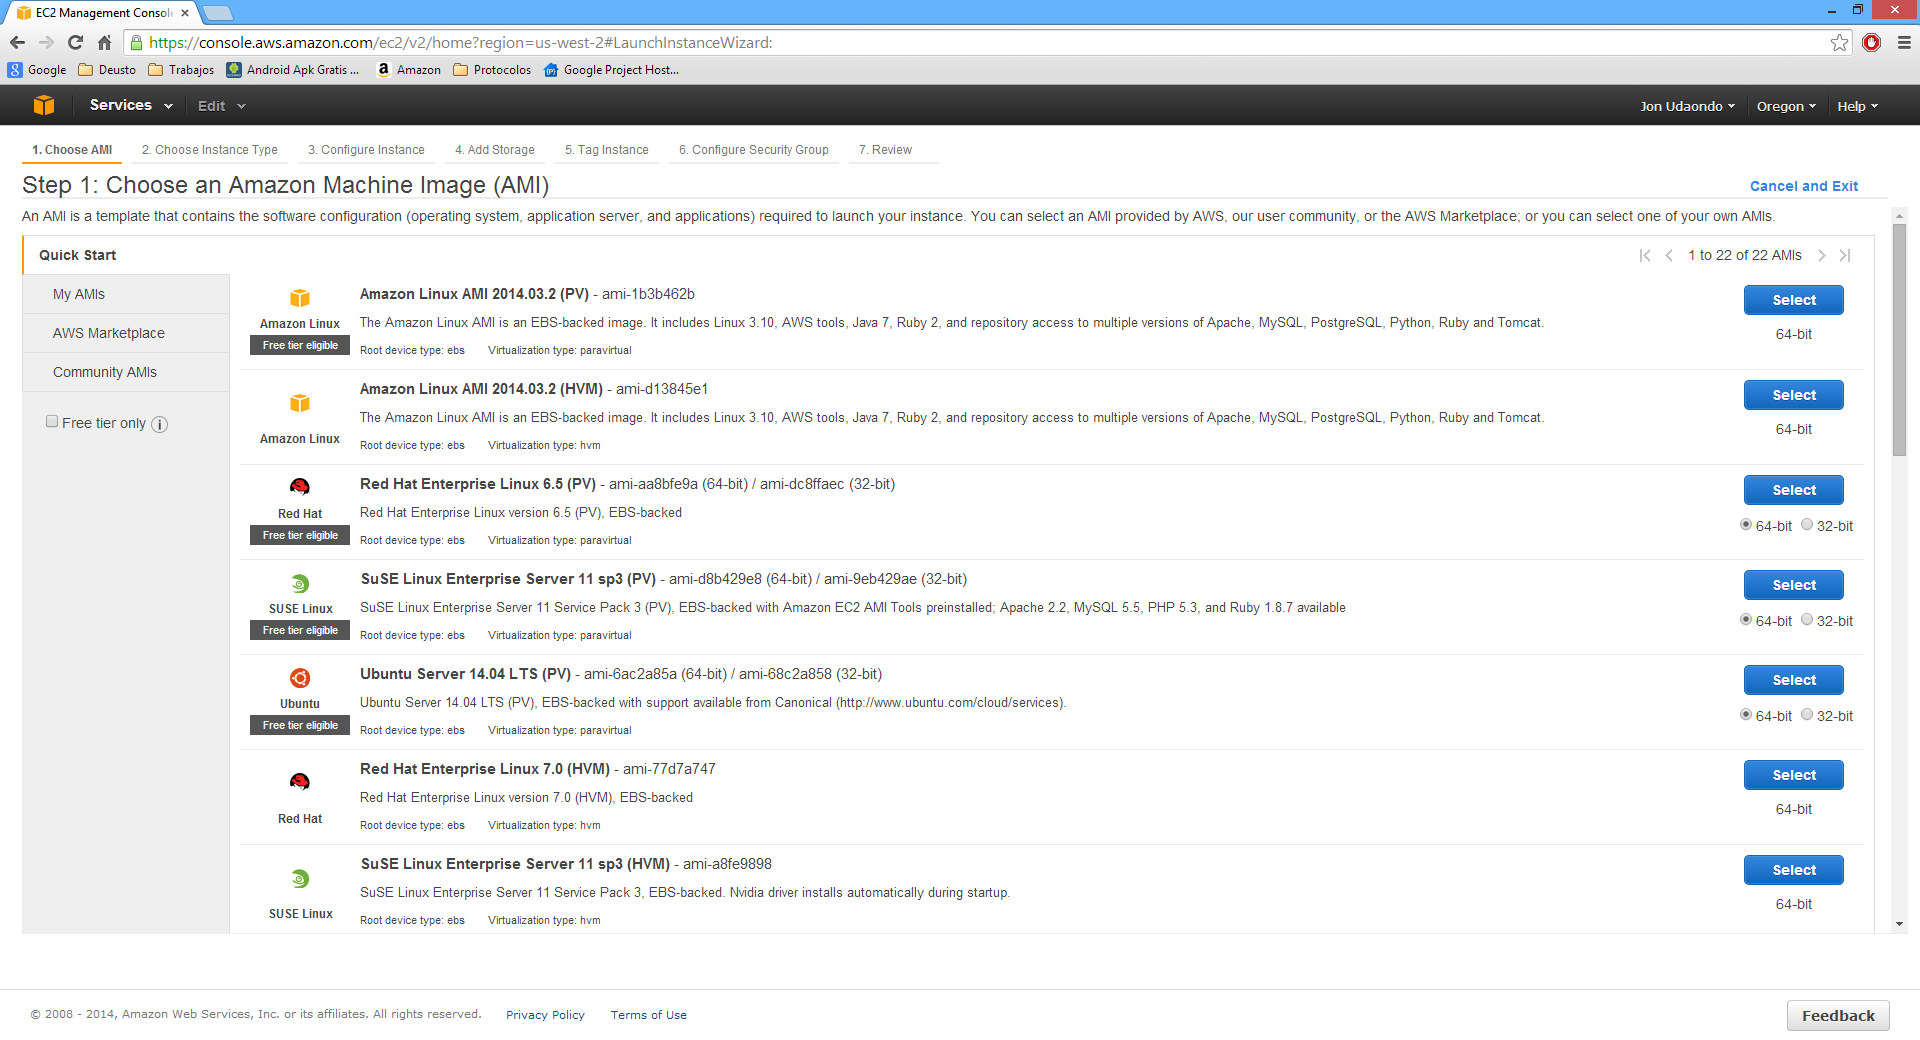
\includegraphics[width=0.8\textwidth] {ami.png}
		\caption{Amazon Machine Image}
		\label{fig: ami}
	\end{figure}
	\item A la hora de seleccionar la instancia elegiremos ``t1.micro'' de la familia ``Micro instances'' y damos a next.
	\item Ahora estaremos en Step 3: Configure Instance Details. Saldrá number of instances (que solo queremos 1), Network, Subnet, Public IP... Dejamos todo tal y como está y damos a ``Next: Add Storage''. 
	\item Step 4: Add Storage. Lo dejamos todo tal y como está con 8GB de tamaño y pulsamos ``Next: Tag Instance''. 
	\item Step 5: Tag Instance. Dejamos tal y como está y damos a ``Next: Configure Security Group''.
	\item Step 6: Configure Security Group. Aquí añadiremos otra regla de seguridad. Para ello con ``Create new security group'' pulsado le damos a ``Add Rule'' y elegimos HTTP.  Tendría que quedar como en la imagen \ref{fig: security_group}. Finalmente pulsamos en ``Review and Launch''.	
		\begin{figure}[htb!]
		\centering
		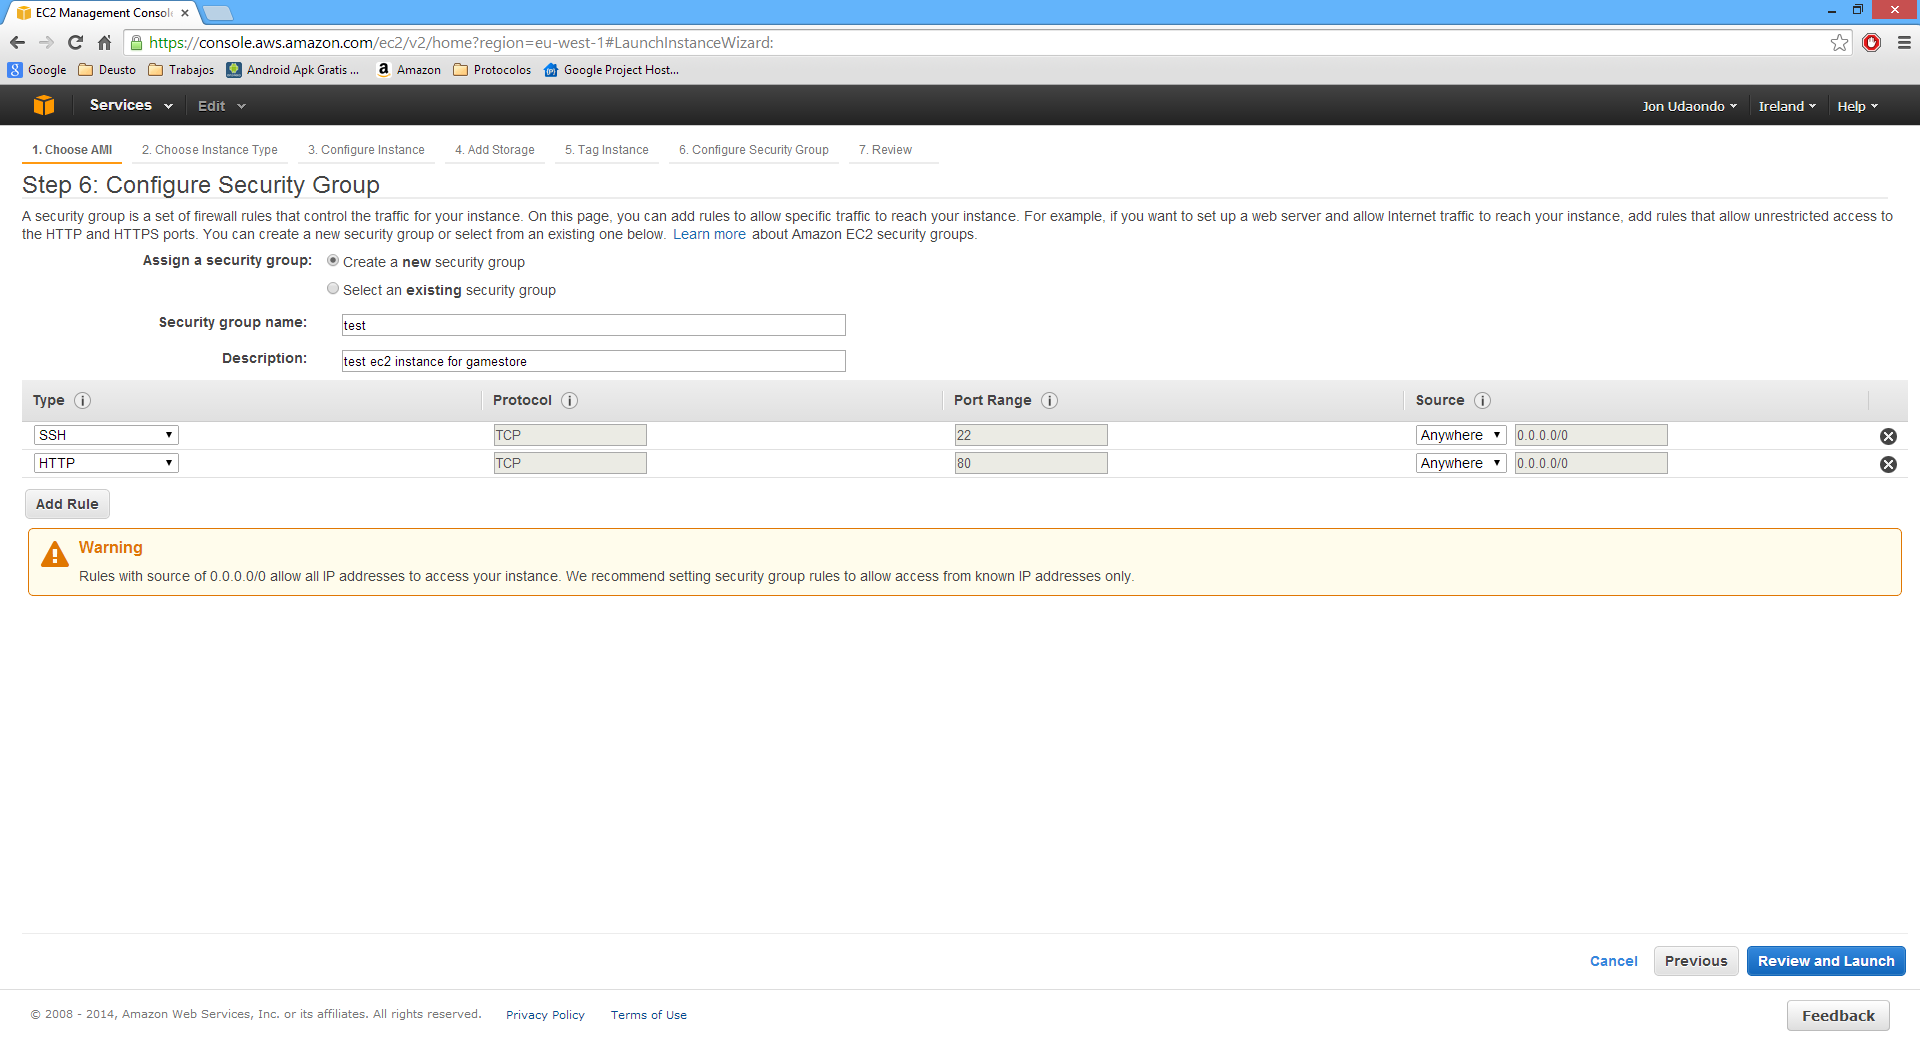
\includegraphics[width=0.8\textwidth] {security_group.png}
		\caption{Step 6: Configure Security Group}
		\label{fig: security_group}
	\end{figure}
	\item Step 7: Review Instance Launch. Si todo ha salido bien deberemos ver algo como esto (fig. \ref{fig: review}). Pulsamos ``Launch''.
	\begin{figure}[htb!]
		\centering
		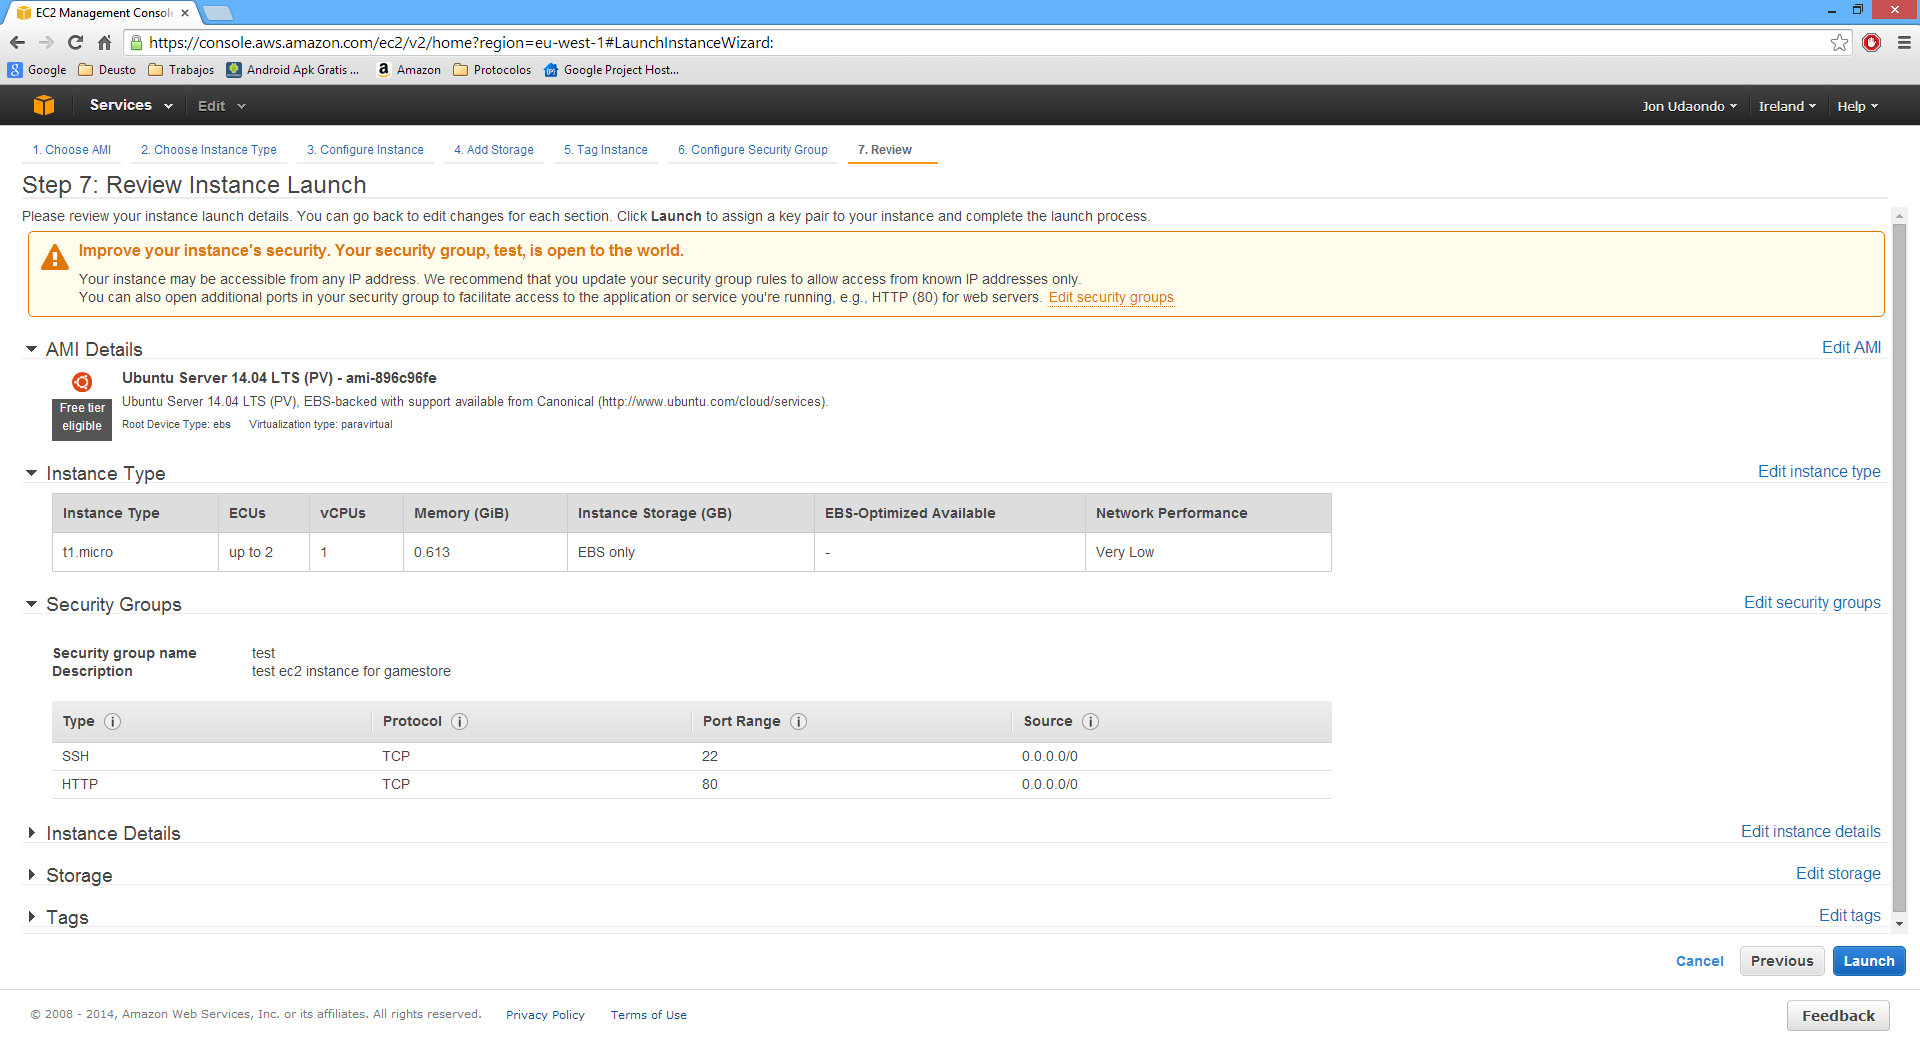
\includegraphics[width=0.8\textwidth] {review.png}
		\caption{Step 7: Review}
		\label{fig: review}
	\end{figure}
	\item Aquí generaremos una Key Pair. Nosotros la llamaremos gamestore. Le damos a Download y ``GUARDAR BIEN ESTE ARCHIVO'', si se pierde puede que no podamos acceder ala máquina virtual en el futuro (fig. \ref{fig: keypair}). El archivo que se bajará tiene la extensión .perm. Finalmente pulsamos ``Launch Instances''.
	\begin{figure}[htb!]
		\centering
		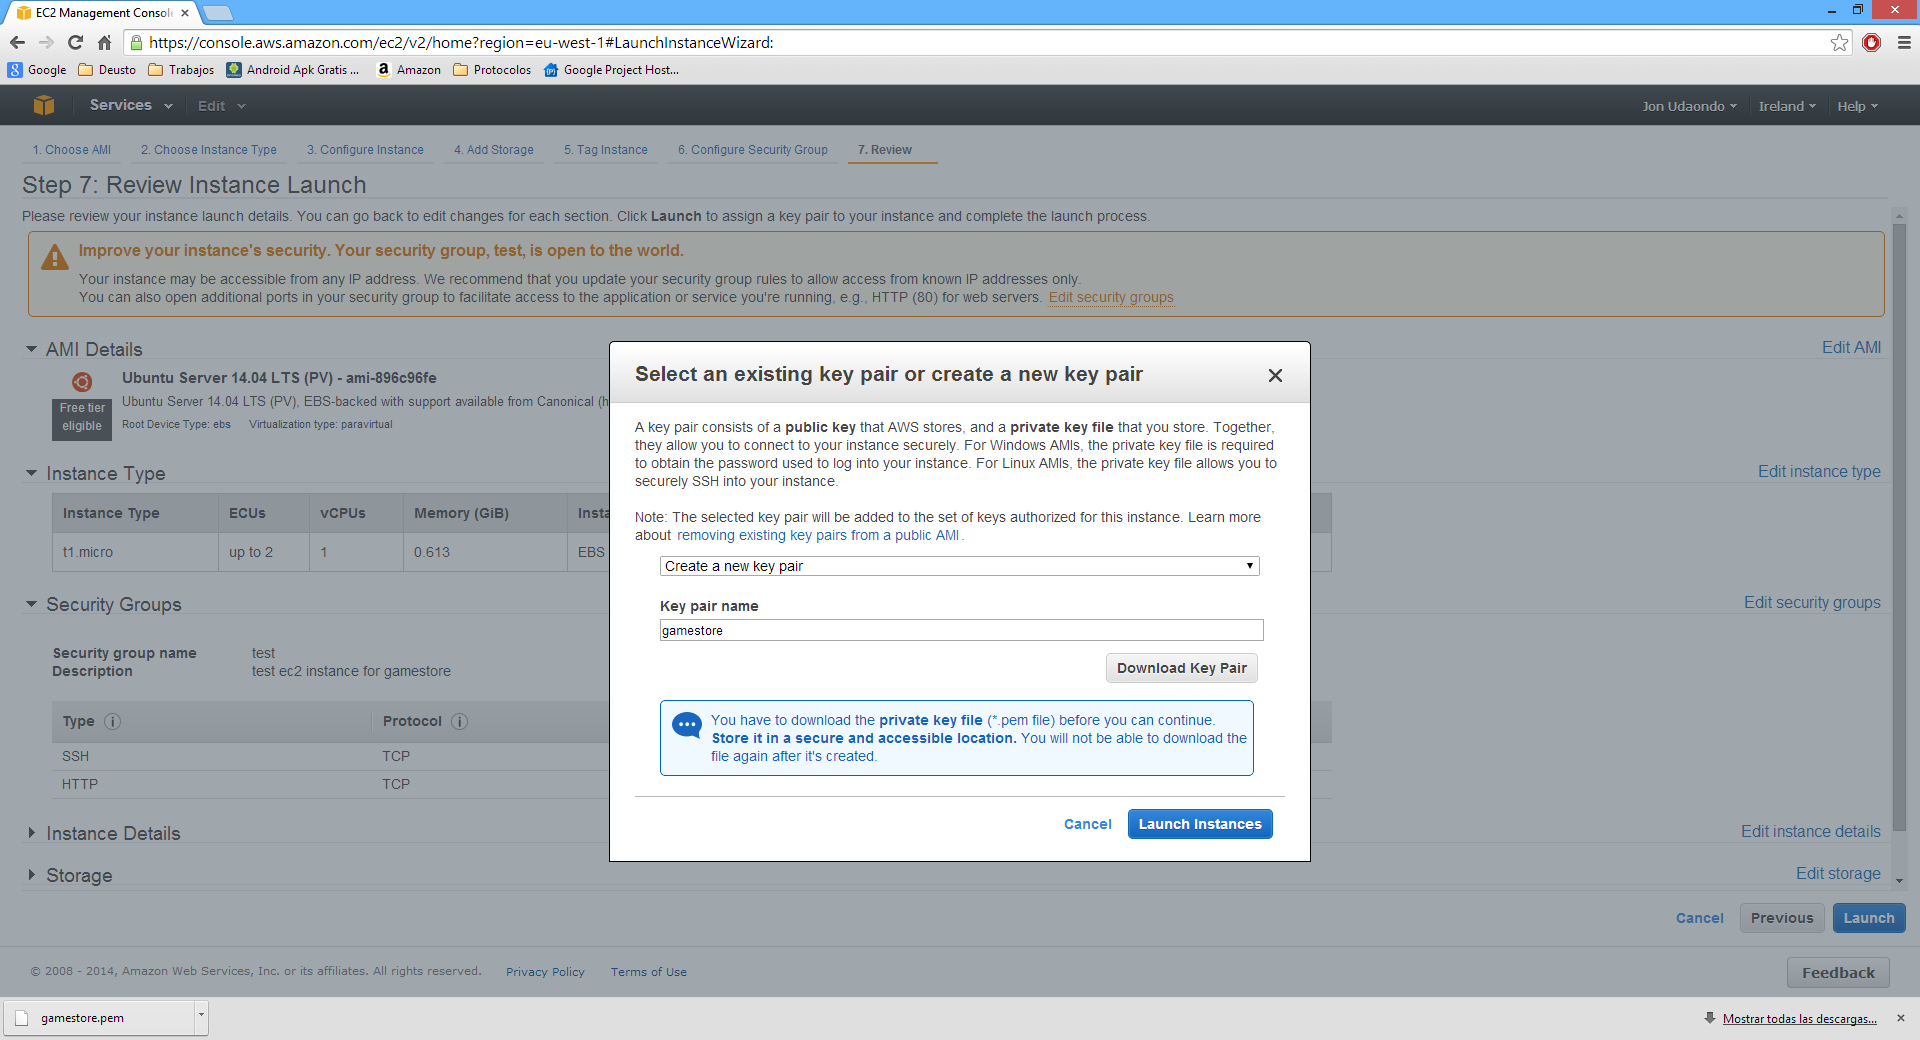
\includegraphics[width=0.8\textwidth] {keypair.png}
		\caption{Creating a new Key pair}
		\label{fig: keypair}
	\end{figure}
	\item Aquí veremos algo asi (fig. \ref{fig: succes}) que significa que la máquina virtual se ha creado satisfactoriamente. Ahora nuestra instancia será visible.
	\begin{figure}[htb!]
		\centering
		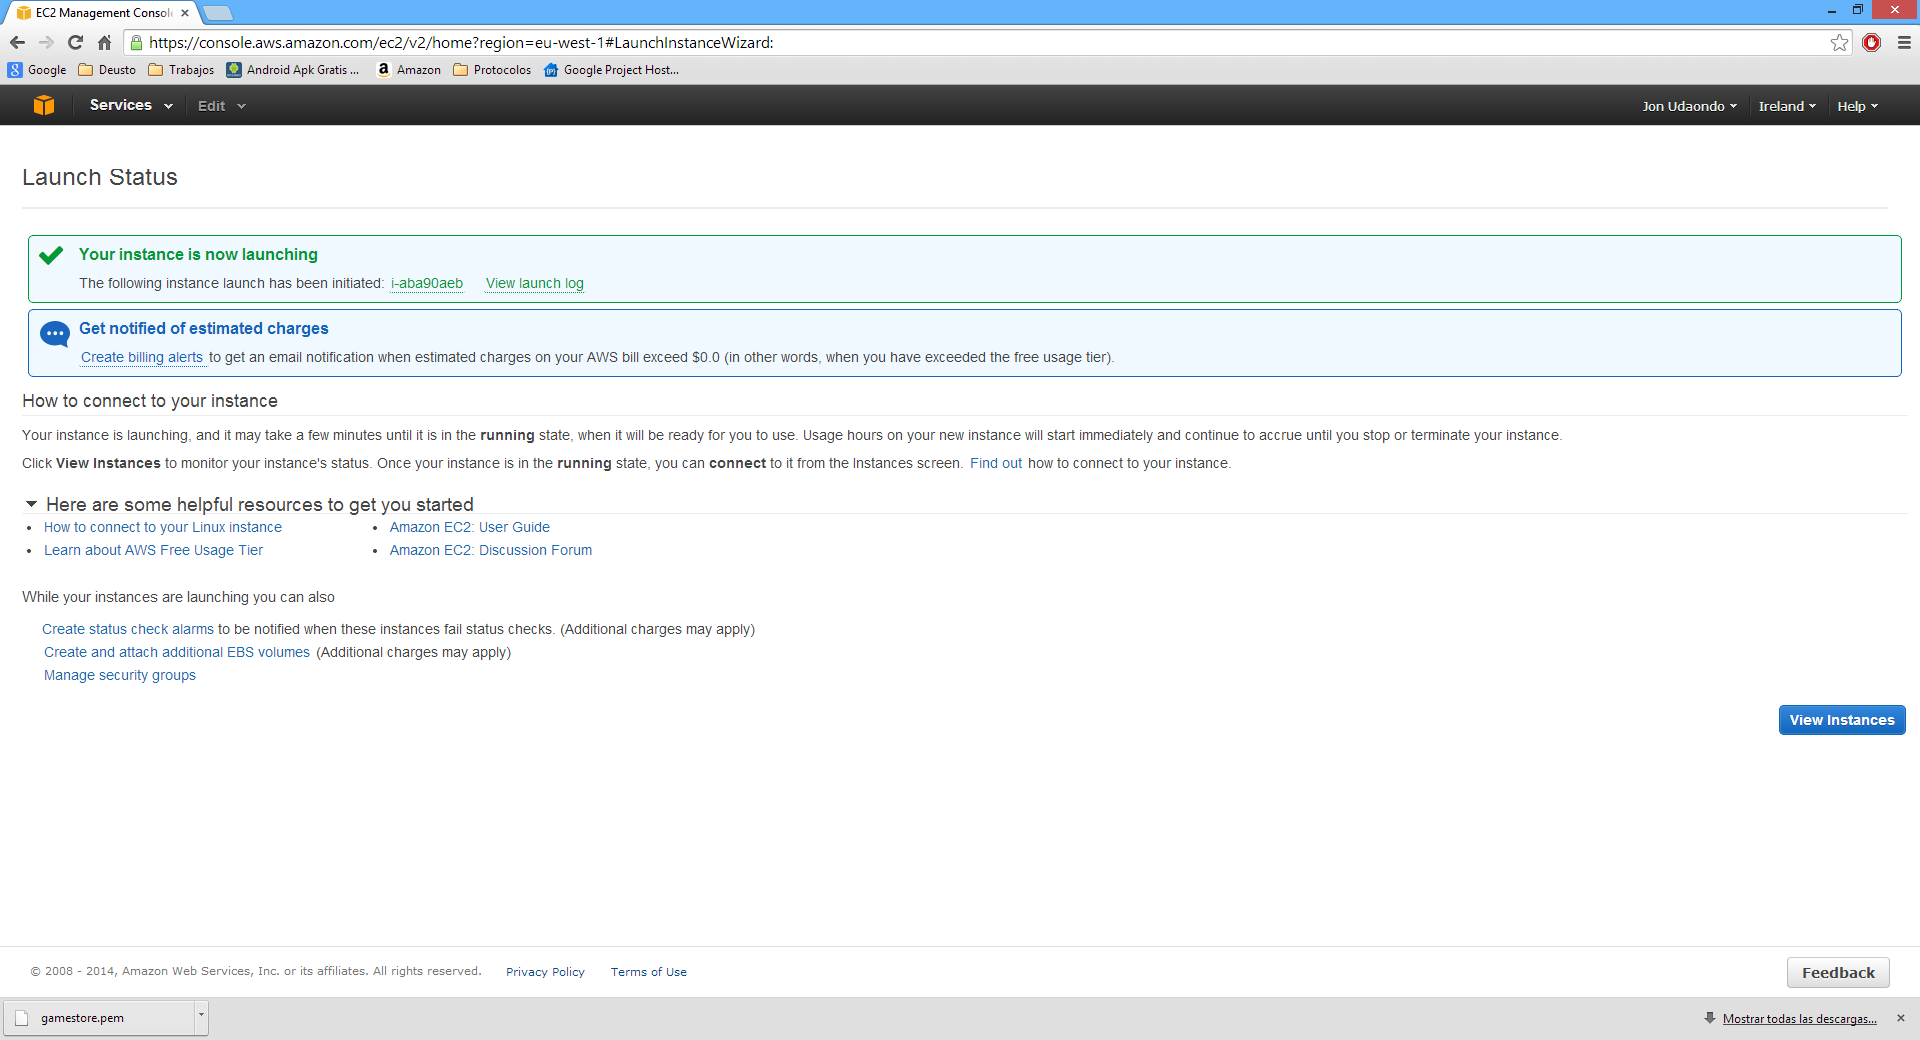
\includegraphics[width=0.89\textwidth] {success.png}
		\caption{Launch status}
		\label{fig: succes}
	\end{figure}
\end{enumerate}

\subsection{Configurando la máquina virtual}
Una vez creada la máquina virtual, volvemos a ``Home'' (\url{https://console.aws.amazon.com/ec2/v2/home?region=eu-west-1}) y en resources veremos que tenemos ``1 running instance''. Pues clickamos ahí seleccionaremos nuestra instancia y le daremos a ``Connect''. Veremos un PopUp en los que nos dirá los pasos que debemos realizar, entre ellos instalar \emph{PuTTY}\footnote{PuTTY, \url{http://docs.aws.amazon.com/AWSEC2/latest/UserGuide/putty.html}} (fig. \ref{fig: connect}).
	\begin{figure}[htb!]
		\centering
		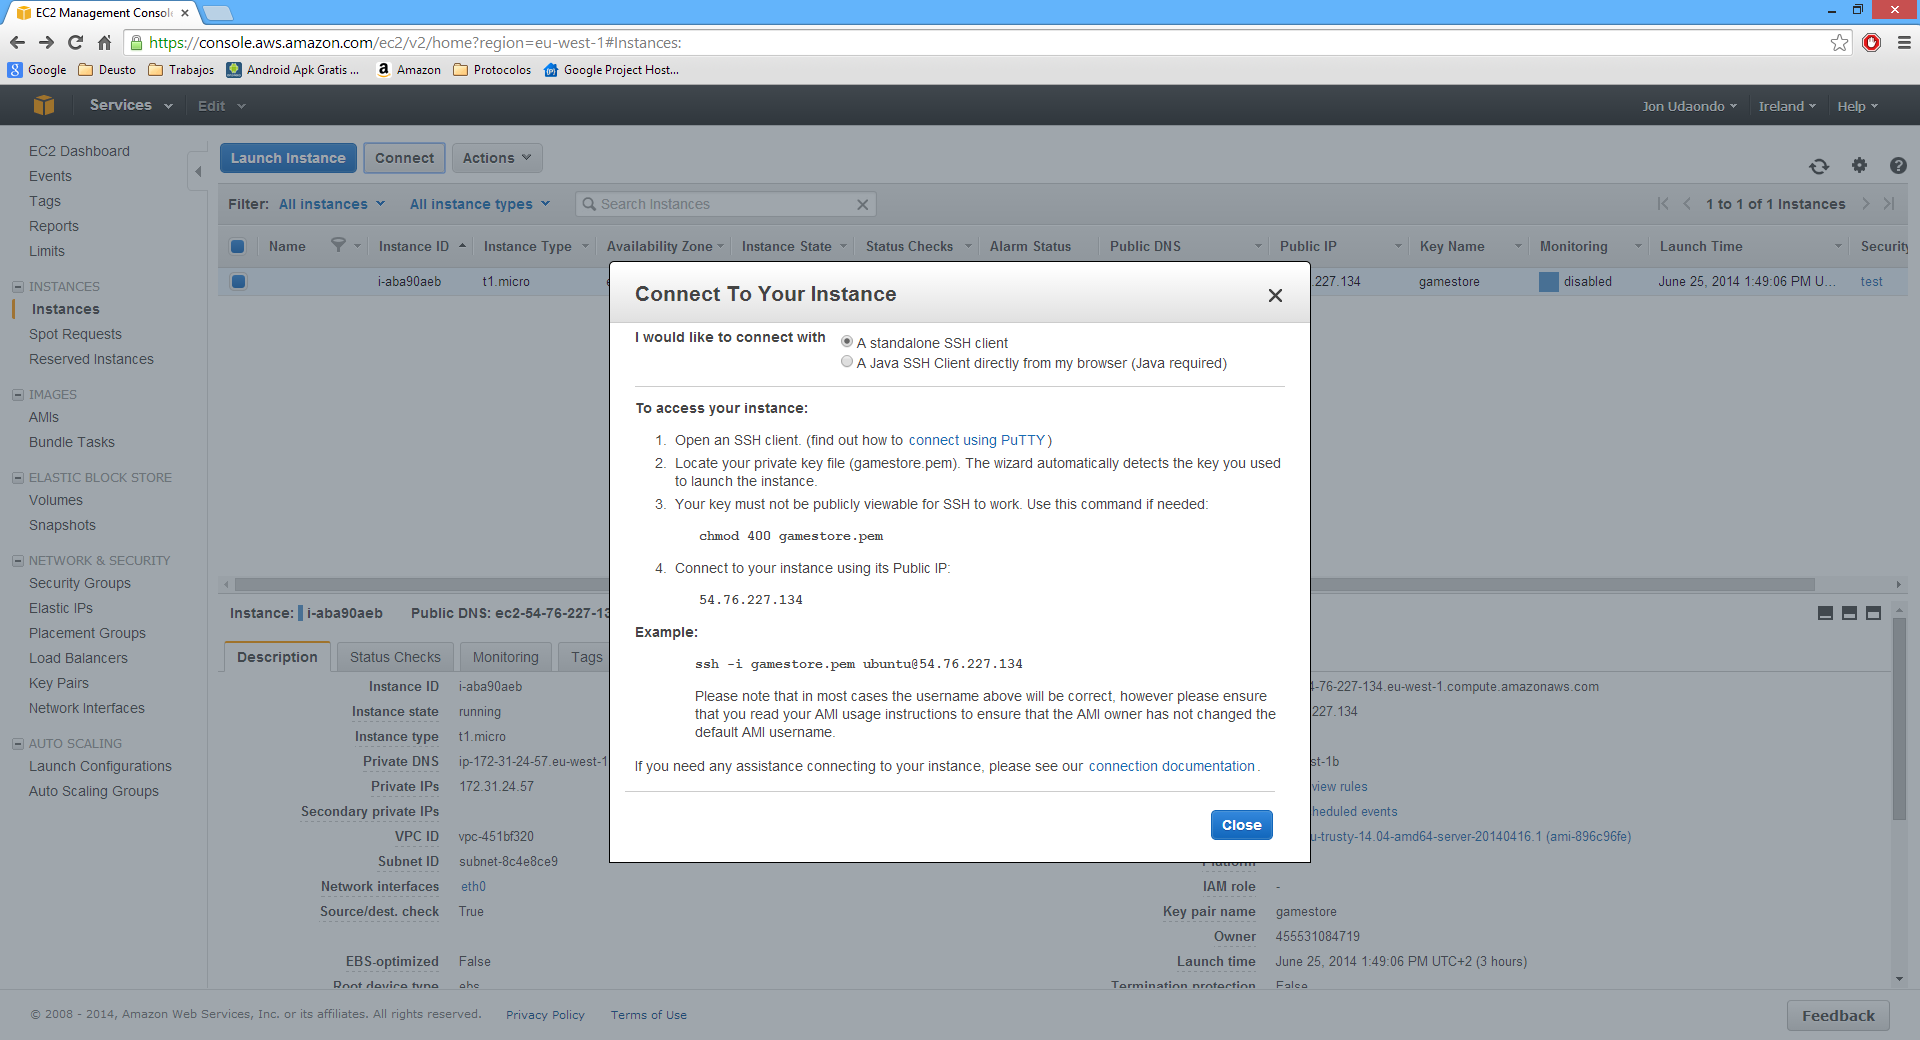
\includegraphics[width=0.8\textwidth] {connect.png}
		\caption{Connect}
		\label{fig: connect}
	\end{figure}
	
\subsubsection{Trabajando con Putty}	
\begin{enumerate}
	\item Nos descargamos PuTTYgen y PuTTY desde \url{http://www.chiark.greenend.org.uk/~sgtatham/putty/download.html}.
	\item Ahora seguimos los pasos que salen en: \url{http://docs.aws.amazon.com/AWSEC2/latest/UserGuide/putty.html}. Al final nos tendría que quedar algo así (fig. \ref{fig: puttyconf}).
	\begin{figure}[htb!]
		\centering
		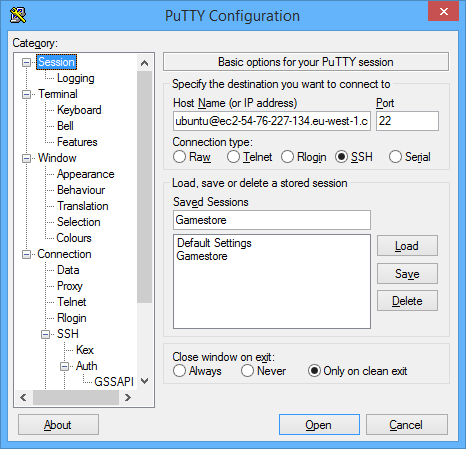
\includegraphics[width=0.7\textwidth] {putty_conf.png}
		\caption{Putty Configuration}
		\label{fig: puttyconf}
	\end{figure}
	\item Una vez configuramos PuTTY y le damos a open veremos algo así (fig. \ref{fig: ubuntuterminal}):
	\begin{figure}[htb!]
		\centering
		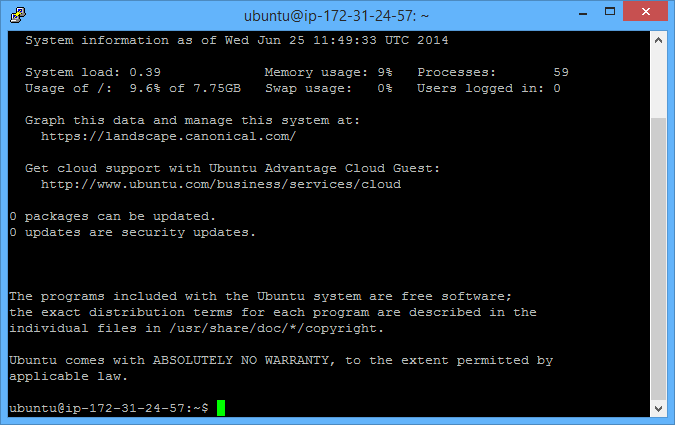
\includegraphics[width=0.7\textwidth] {ubuntuterminal.png}
		\caption{Ubuntu Terminal}
		\label{fig: ubuntuterminal}
	\end{figure}
\end{enumerate}

\subsection{Desplegando la aplicación}
Una vez que estamos en terminal procederemos a instalar los recursos necesarios para el despliegue de nuestra aplicación.	
\begin{enumerate}
	\item Instalando Java 7
	\begin{lstlisting}
	$ sudo apt-get install icedtea-7-plugin openjdk-7-jre
	$ sudo apt-get install openjdk-7-jdk
	\end{lstlisting}
	\item Instalando Apache Tomcat, PHP y MySQL
	\begin{lstlisting}
	$ sudo apt-get install tomcat7
	$ sudo apt-get install tomcat7-admin
	$ sudo apt-get install php5 mysql-server php5-mysql
	\end{lstlisting}
	\item Reiniciamos el servidor Apache para ver que funciona correctamente
	\begin{lstlisting}
	$ /etc/init.d/tomcat7 restart
	\end{lstlisting}		
	\item Veremos que tras instalar Apache 2 e introducir el DNS publico (\url{http://ec2-54-76-227-134.eu-west-1.compute.amazonaws.com}) no funciona. Esto es porque Tomcat trabaja en 8080. Y vemos que si introducimos \url{http://ec2-54-76-227-134.eu-west-1.compute.amazonaws.com:8080} tampoco funciona. Eso es porque en las politicas de seguridad tenemos que añadir el puerto 8080. En el video de la referencia 3 se explica perfectamente. 
	Una vez establecida la política se debería de ver mítica página de It Works!
	\item Ahora intentaremos cambiar y redirigir el puerto 8080 al DNS para que no tengamos que introducir 8080 (Hacerlo como root).
	\begin{lstlisting}
	$ iptables -t nat -I PROROUTING -p tcp -dport 80 -j REDIRECT --to-port 8080
	$ iptables-save
	\end{lstlisting}	
	\item Nos dirigimos a ``'/etc/tomcat7/tomcat-users.xml' y generamos derechos para manegar webapps e insertamos la siguiente linea.
	\begin{lstlisting}
	< user username=''admin'' password=''admin'' roles=''manager-gui,admin-gui''/>
	\end{lstlisting}
	\item Reiniciamos el servidor Apache para ver que funciona correctamente
	\begin{lstlisting}
	$ /etc/init.d/tomcat7 restart
	\end{lstlisting}	
\end{enumerate}


	
\pagebreak
\begin{thebibliography}{20}
 \bibitem{1} \textsc{Pase de parametros del Jsf al Servidor}:
 \textit{\url{http://java-adictos.fitsoft.com.ve/2013/01/pase-de-parametros-del-jsf-al-servidor.html}}
 \bibitem{2} \textsc{JSF 2 Repeat Tag Example}:
 \textit{\url{http://www.mkyong.com/jsf2/jsf-2-repeat-tag-example/}}
 \bibitem{3} \textsc{Amazon EC2, Apache, MySQL, PHP, and Tomcat 7 Tutorial}:
 \textit{\url{https://www.youtube.com/watch?v=pZFSSVVdqmw}}
 \bibitem{4} \textsc{Tutorial : Deploy an .war(java web application) in apache tomcat server (part2)}:
 \textit{\url{https://www.youtube.com/watch?v=75dTrFKr538}}
 \bibitem{5} \textsc{How to Setup Amazon Web Services EC2 Instance with Apache, PHP, MySQL}:
 \textit{\url{https://www.youtube.com/watch?v=wNr7YqjjzOY}}
 \bibitem{5} \textsc{Tutorial de uso de Amazon EC2. Creando maquina virtuales gratis}:
 \textit{\url{http://www.bandin.info/2012/04/manual-de-uso-de-amazon-ec2-creando-maquina-virtuales-gratis/}}



\end{thebibliography}


\end{document}